\chapter{System Model and Algorithm}
In this chapter, our proposed system model and algorithm will be discussed. We proposed a system diagram. The system core is an IoT based devices that will collect data from patients and send them to server. In server the collected data will be processed via a machine learning algorithm. We will use Attention RNN algorithm and also use some classifier like SVM, RF to detect fall from the camera based image and adding a smart home automation system to give a short moment comfort to the patients with notifying at emergency.
\section{Proposed System Architecture}


We have proposed the systems architecture mentioned in Figure 3.1 contains the full system work flow.

\begin{figure}[ht]
   \centering
   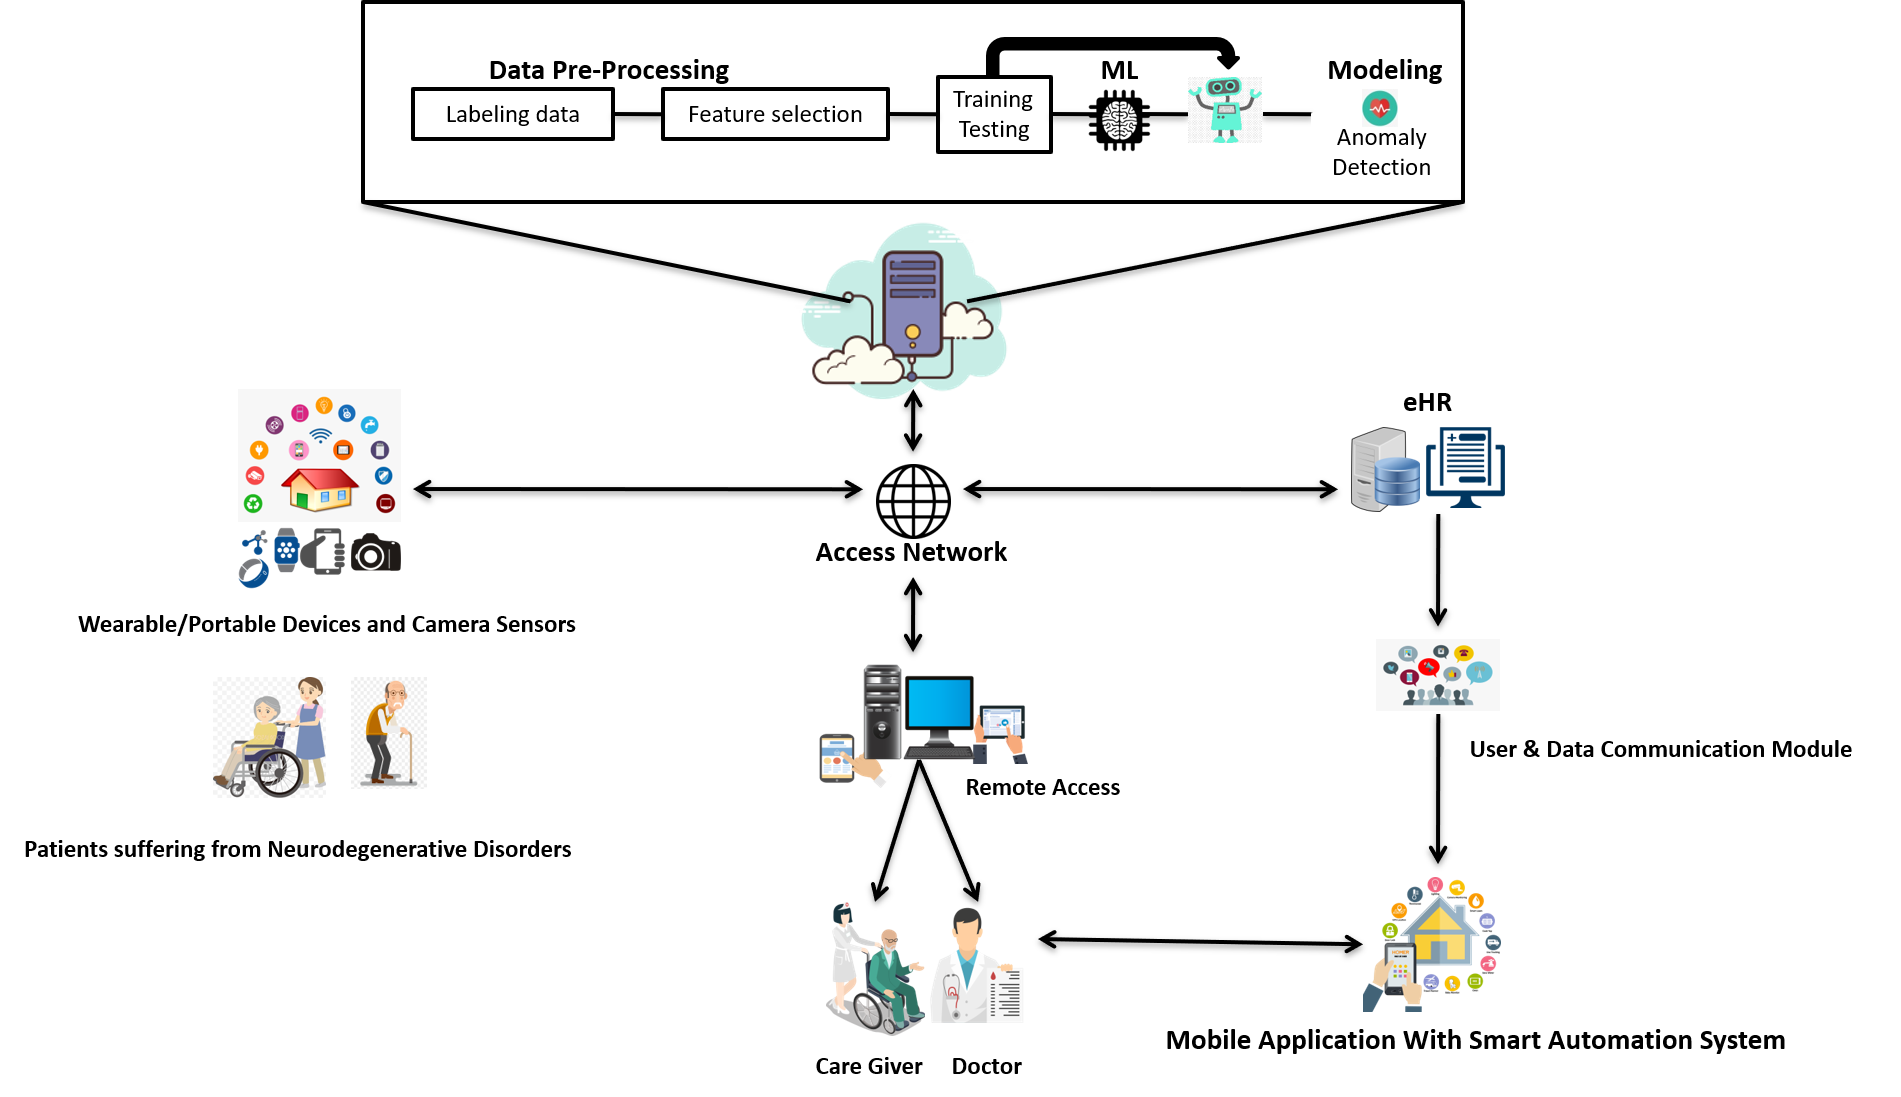
\includegraphics[width=5.5in]{Chap3/Picture4.png}
   \caption{Proposed System Model}
   \label{fig:model}
\end{figure}

\vspace{0.5cm}
Here, the platform we will use an e-health sensor in our wearable device as a platform for its full compatibility with raspberry pie and Arduino Microcontroller and it also can be powered by the PC or by the external power supply. %First, we need to make a wearable device. 
Our wearable device integrated with various sensors like-  
DHT 11 temperature and humidity sensor collects the data of temperature or humidity, MPU 6050 Accelerometer Gyroscope collects data of action like shaking and spinning, Glucometer determines approximate blood glucose concentration and calculates the blood glucose level, Galvanic Skin Response sensor (GSR) collects the data whether sweating or not, Sphygmomanometer collects blood pressure rate, ECG Sensor (AD8232 Module) collects the data of the electrical and muscular functions of the heart, Optical Pulse Sensor collects the pulse rate data, Pulse Oximetry collects the data of the percentage of hemoglobin and protein in blood and oxygen saturation. After collecting the data via sensor, then data is transmitted across the network to the cloud server. % There will be also a Wi-Fi module connected to the Microcontroller. The GPS tracker send the patient’s current location to the cloud server via Wi-Fi or cellular network. 
 Smart automation system will also be integrated to the module. Here, voice and video instruction can be also sent to the patient by the caretakers and doctors for making patient’s life a bit easier and comfortable.
 
%  The flow chart of the working procedure of IoT system is illustrated in \ref{fig:Working Procedure Of IoT}.
 
%  \begin{figure}[ht]
%     \centering
%     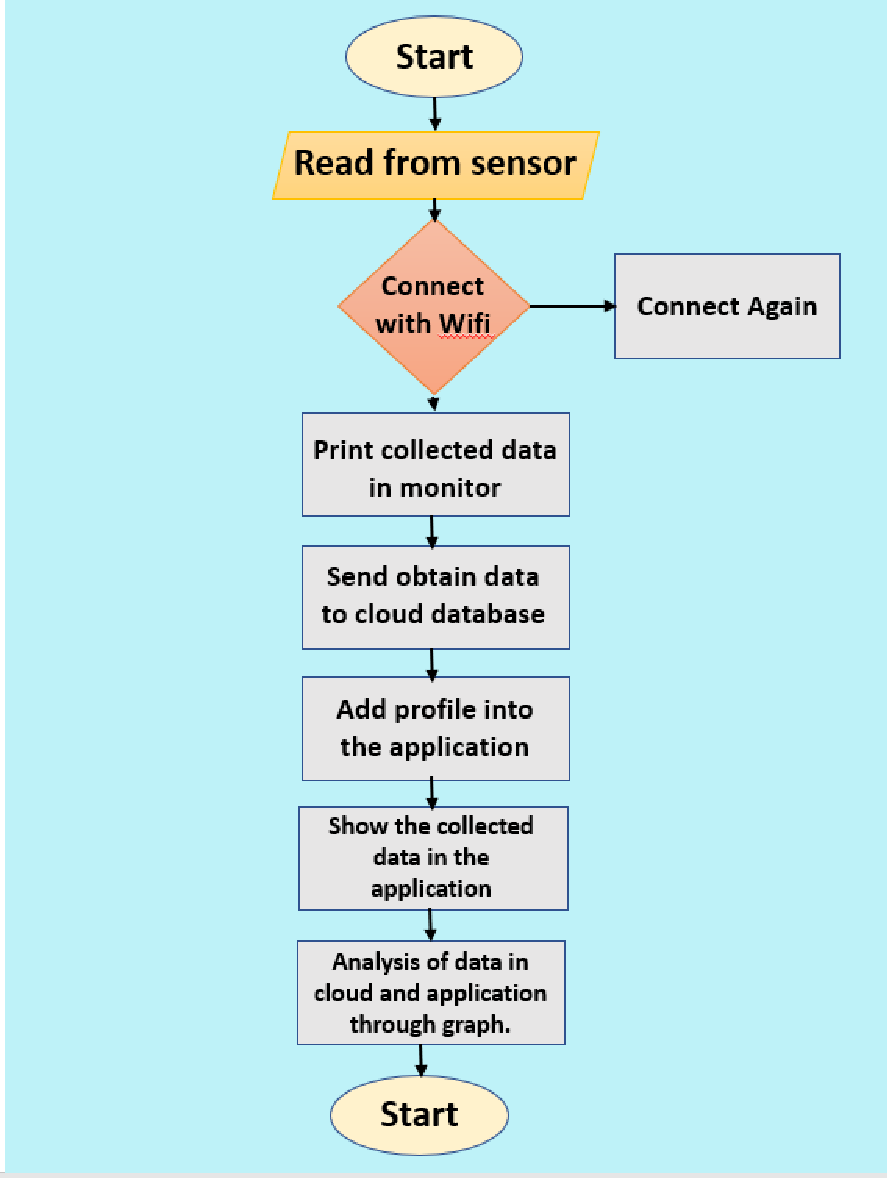
\includegraphics[scale=0.5]{Chap3/IoT.pdf}
%     \caption{Working procedure of IoT system}
%     \label{fig:Working Procedure Of IoT}
% \end{figure}
 
 \vspace{0.5cm}
 We use deep learning algorithms for the interpretation of the gathered data and for the processing as well as for supporting the patient's framework in decision making. For doing this first we need to label the collected data for feature extraction in the data pre-processing. Then we train the system for detecting the diseases and test it. This helps us to determine which data we can store and which we do not choose. Repeated data will not be preserved here. So, It will decrease the storage size. Thus, memory will be used effectively. After that constructive the patient's medical report will be sent to the mobile application. In the mobile application, specified doctors and care takers can see the particular patient’s health conditions by creating their personal profile. If the patient’s condition is not so well or in the emergency the application will send an alert to the doctors and caretaker. Meanwhile smart automation system will be automatically activated if it’s needed. Such as, if patient will sweat so much, the fan will be automatically turned on. Again, if patient’s temperature will rise high, the fan will be automatically turned off and so on. The smart automation system can also be accessed via mobile application by the specified doctors and caretakers.  
With our system we can monitor the patient all the time locally or remotely. In the patient’s sudden illness there will be always someone to help him. The patient can be monitored at home easily and the signals are sent to a hospital or the dearest person through the available communication line easily. Our mobile application makes information exchange between doctors and patients or between institutions in a simpler way. This lowers the costs, expands the spectrum and extends to all forms of medical services and increases service quality.
The flow chart of the proposed fall detection process is illustrated in \ref{fig:fallchart}

\begin{figure}[ht]
    \centering
    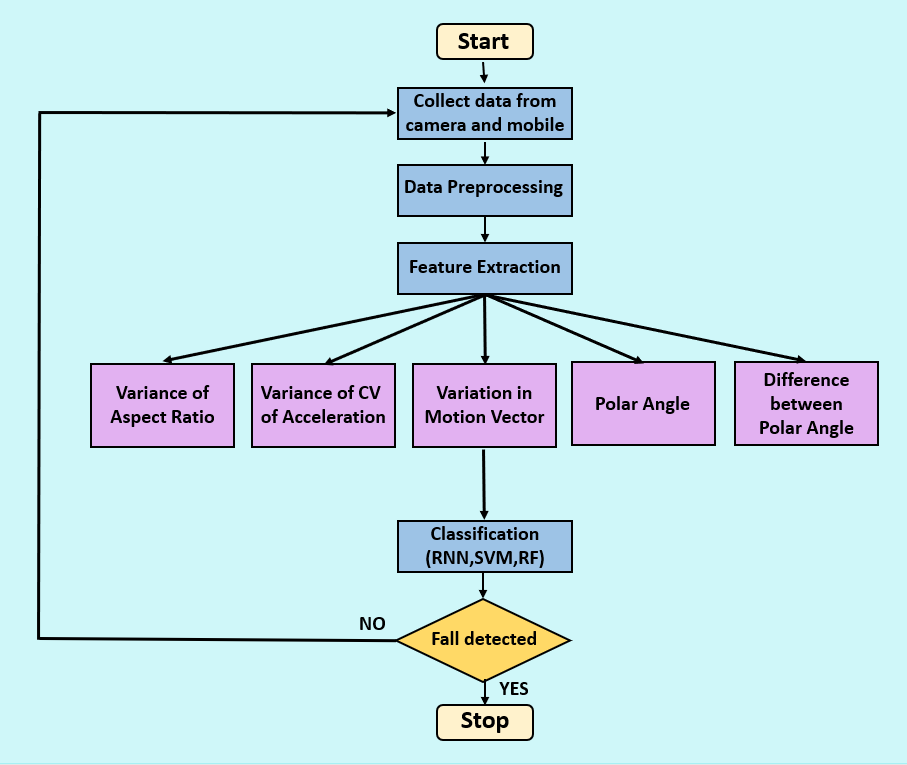
\includegraphics[scale=0.5]{Chap3/Capture.PNG}
    \caption{Flowchart for proposed fall detection system}
    \label{fig:fallchart}
\end{figure}

% \section{Components of IoT System}
% Here we will discuss about the required components of the IoT system. The hardware and software components those we have used here are: node mcu ESP 8266, breadboard, Arduino coding, programming language C,java,xml, various types of cables, dh11 temperature humidity sensor, 128*64 |2C OLED display, Arduino software, Thingspeak IoT cloud platform, Android Studio, Arduino IDE etc. A brief description of these are as follows:

% \subsection{Hardware Components}
% \textbf{Node mcu ESP 8266:} NodeMCU is an open source IoT platform including firmware which runs on the ESP8266 Wi-Fi SoC from Espressif Systems, and hardware which is based on the ESP-12 module. The term "NodeMCU" by default refers to the firmware rather than the development kits. The firmware uses the Lue scripting language.

% \begin{figure}[ht]
%     \centering
%     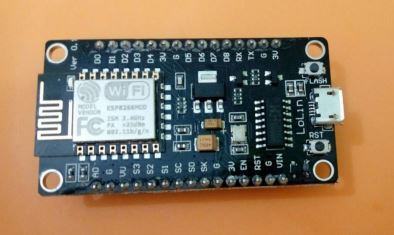
\includegraphics[scale=0.9]{Chap3/arduino.JPG}
%     \caption{Node MCU ESP 8266}
%     \label{fig:fallchart}
% \end{figure}

% The ESP8266 is a low-cost Wi-Fi chip with full TCP/IP stack and microcontroller capability produced by Shanghai-based Chinese manufacturer, Espressif.

% \textbf{ESP8266 Feature:}
% \begin{itemize}
%     \item Open Source
%     \item Interactive
%     \item programmable
%     \item Low cost
%     \item Simple
%     \item Smart
%     \item WI-FI enabled
%     \item USB-TTL included
%     \item Plug and Play
% \end{itemize}


% \textbf{Node MCU DEVKIT 1.0 Specification:}
% \begin{itemize}
%     \item \textbf{Developer :} ESP8266 Open source Community
%     \item \textbf{Type :}Single-board microcontroller
%     \item \textbf{Operating System: }XTOS
%     \item \textbf{CPU: }ESP8266
%     \item \textbf{Memory: }128kBytes
%     \item \textbf{Storage: }4MBytes
%     \item \textbf{Power By: }USB
%     \item \textbf{Power Voltage: }3v ,5v (used with 3.3v Regulator which inbuilt on Board using Pin VIN)
%     \item \textbf{Code: }Arduino, Cpp
%     \item \textbf{Arduino Used: }Arduino IDE
%     \item \textbf{GPIO: } 10
% \end{itemize}
% \vspace{.5cm}
% \textbf{DHT11 temperature humidity sensor:}
% This DHT11 Temperature and Humidity Sensor features a calibrated digital signal output with the temperature and humidity sensor complex which ensures the high reliability and excellent long-term stability. It has excellent quality, fast response, anti-interference ability and high cost performance advantages.

% \begin{figure}[ht]
%     \centering
%     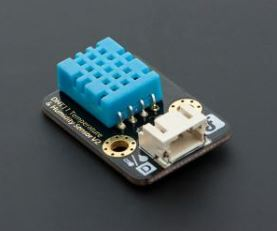
\includegraphics[scale=0.9]{Chap3/humidity sensor.JPG}
%     \caption{DHT11 temperature humidity sensor}
 
% \end{figure}
% \vspace{.5cm}
% \textbf{MPU 6050 Accelarometer Gyroscope:}
% The MPU-6050 is a popular six DoF accelerometer and gyroscope (gyro) that has all the info you need on how things are shaking and spinning .

% \vspace{.5cm}
% \textbf{Sphygmomanometer: } It is a sensor which measures blood pressure used with a stethoscope when using the auscultatory technique. 

% \vspace{.5cm}
% \textbf{Pulse Oxymetry: } It tests the oxygen saturation level in the blood of a patient. This system consists of a source of red and infrared light, photo detectors and a probe to relay light, usually a fingertip or earlobe, through a transparent, vibrating coronary artery bed. 

% \vspace{.5cm}
% \textbf{ECG Sensor: } Up to twelve electrodes are connected to the chest and limbs of patients during an ECG. Sticky patches with wiring that attach to a display are the electrodes. The electrical signals of patient's heart beat are registered. A machine monitors the data and shows it on a display or on document as waves patterns. 

% \vspace{.5cm}
% \textbf{Galvanic Skin Response Sensor(GSR) : } It leads to changes in the composition of the sweat
% gland that represent the strength of our emotional state, otherwise known as emotional arousal. It can measure data about our sweat secretion which affects a major part in health management.

% \vspace{.5cm}
% \textbf{Glucometer: } It can measure the glucose level in blood of a patient. People having diabetes need to be monitored their condition by using Glucometer. 


% \vspace{.5cm}
% \textbf{Optical Pulse Sensor: } Optical pulse sensors are used to monitor patient's heart rate. 

% \vspace{0.5cm}
% \textbf{2C OLED display: } 
% This display is made of 128x64 individual white OLED pixels, each one is switched on or off by the controller 
% Chip. Less power is required to work and so it has such a high contrast. A 3.3V power supply and 3.3V logic levels for communication are required by the OLED itself.

% \vspace{0.5cm}
% \textbf{Arduino IDE: }
% Arduino is an open-source platform used in electronics programs for design. The Arduino consists of both a programmable physical circuit board (often referred to as a Microcontroller) and a software part, or IDE (Integrated Development Environment) that is
% used for writing and transferring machine code to the physical board while running on the computer. In comparison, a simpler version of C++ is used in the Arduino IDE, make programming simpler to understand.


% % \textbf{Reset Button} By pushing a reset button of arduino it restart any reloaded code while need to avoid any kind of repeatation.

% % \textbf{Power LED Indicator: } Just underneath and to one side of "UNO" on our circuit board, there's a little LED close to 'ON'. On the off chance that this light doesn't turn on, there's a decent possibility something isn't right and should recheck it.

% % \textbf{TX RX LEDs: }TX is short for transmit, RX is short for receive. These markings appear quite a bit in electronics
% % to indicate the pins responsible for serial communication. In our case, there are two places on the Arduino UNO where TX and RX appear – once by digital pins 0 and 1, and a second time next to the TX and RX indicator LEDs (12). These LEDs will give us some nice visual indications whenever our Arduino is receiving or transmitting data.

% % \textbf{Voltage Regulator: } The voltage regulator says how to control the amount of voltage that is let into the Arduino. It has a limit of 20 volts.


% \subsection{Software Components}
% \textbf{ThingSpeak: } ThingSpeak helps one to combine, simulate and validate live data which is in the cloud. IoT devices can easily send data to ThingSpeak using most popular IoT protocols. It collects data by sending IoT data privately to the cloud. Then ThingSpeak analyze and simulate the data using MATLAB. In the end it act by triggering a reaction.Based on schedules or activities, ThingSpeak will run our IoT analytics automatically. 

% \vspace{0.5cm}
% \textbf{Android Studio: } Android Studio is a modular building framework focused on Gradle that provides an environment where tablets, Android Phones, Android  Wear, Android Auto, and Android Tv apps can be designed.
% It supports a wide range of layout design with support of drag and drop editing. Besides built in support of google makes this software more popular to the android developers.





\section{Data Pre-processing}
After collecting the data our system will pre-process the dataset for the algorithm. The ML algorithm will compare new data with the trained dataset. Before entering the main algorithm, we have to pre-process the collected new data. To pre-process the collected data, we have used the following algorithm:

\begin{figure}[H]
   \centering
   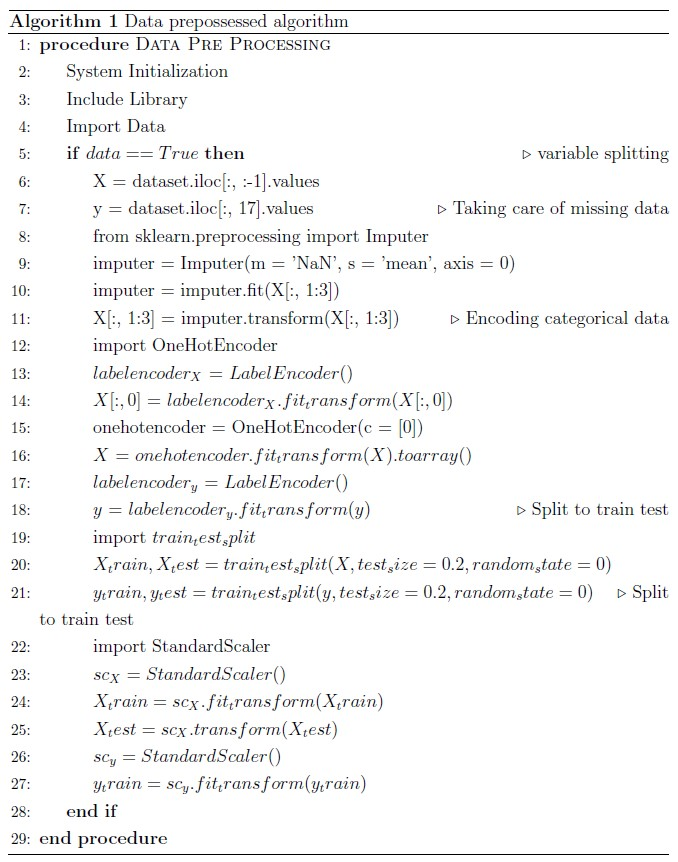
\includegraphics[width=4.3in]{Chap3/algorithm.png}
   
\end{figure}

After data pre-processing we will use Machine learning algorithm, LSTM RNN. 

% \section{ML Algorithm and Classifiers}
% We hit upon a plan to manage Neuro De-generative diseases with our system. We are using the  attention RNN as Machine Learning Algorithm which is a section of RNN. As our data set will be very big we can modify it to Attention RNN algorithm. \cite{arbel_attention_2019}
% \subsection{Attention RNN}
% Recurrent Neural Networks (RNNs) have been effectively used for several sequential data functions, such as machine translation, emotion processing, simulation of time series, image processing etc. Attention is a function combined in the RNN that allows it to concentrate on certain aspects of the input sequence while forecasting a certain portion of the output sequence, making it easier to understand and of better quality. The integration of attention processes has made it possible to enhance efficiency in many functions, making it an important part of modern RNN frameworks.
% The attention function helps the RNN to concentrate on a particular part of the input sentence while the translation is output. Larger attention parameters link the corresponding parts and allow the network to achieve a state.

% The problem with RNN engineering lies in the way the decoder has to communicate to the whole information sequence as a lone vector, which can lead data to be lost. In addition, the decoder has to convert the data passed from this single vector, an arbitrary assignment in itself. While considering Attention RNN halfway fixes this issue. It permits a machine interpreter to investigate all the data the first sentence holds, at that point produce the correct word as per the current word it chips away at and the unique circumstance. It keeps up the data missing issue. As our requirements we use Attention RNN for our project.

% To apply Attention RNN algorithm we have to bear in mind about the following things:
% \begin{enumerate}
%     \item {\textbf{Attention Model: }} Considering an attention model with 4-time steps, having a solitary layer RNN encoder. We mean the yield vectors by h1, h2, h3, h4 and the encoder's information vectors by x1, x2, x3, x4 . The attention function is placed between the encoder and the decoder, its information is considered out of  the conditions of the decoder s0, s1, s2, s3, and the encoder's yield vectors h1, h2, h3, h4, the consideration's yield is a succession of vectors called setting vectors meant by c1, c2, c3, c4.
    
%     \begin{figure}[H]
%   \centering
%   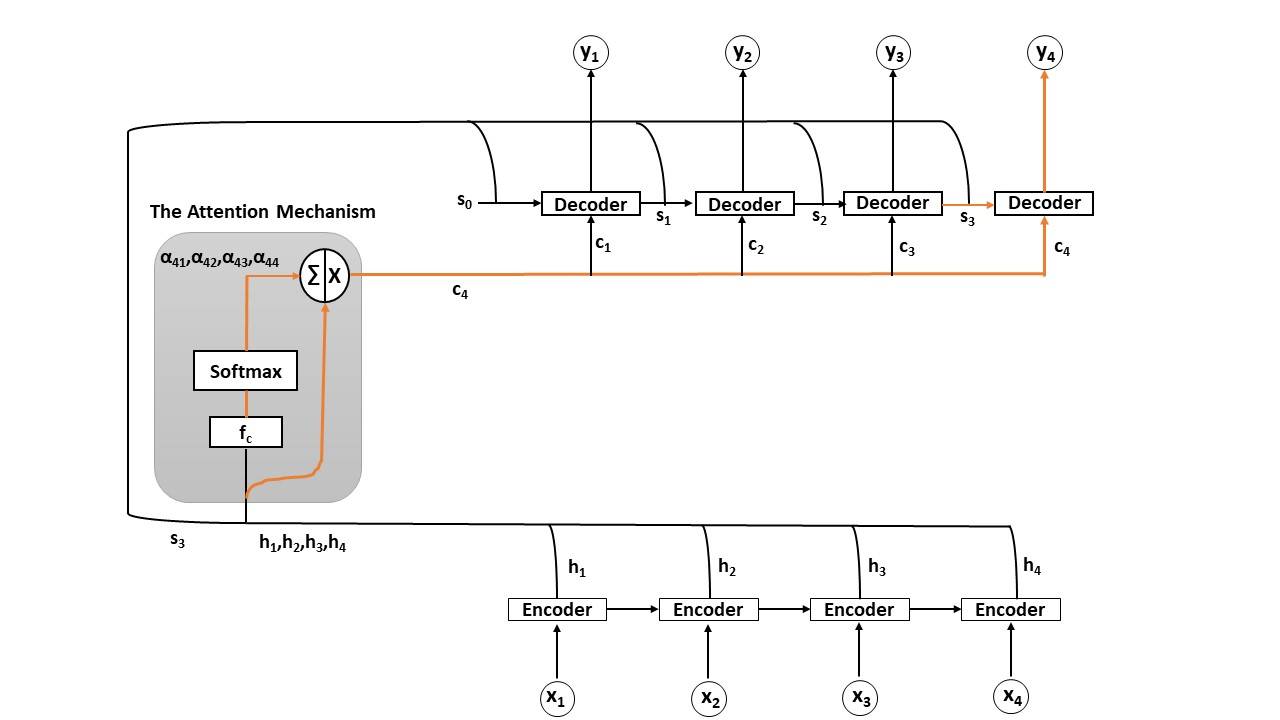
\includegraphics[width=5.4in]{Chap3/pic1.jpg}
%   \caption{RNNs with an attention mechanism}
%   \label{fig:model}
%     \end{figure}
    
%     \item {\textbf{Context Vector: }}The context vectors empower the decoder to zero in on specific pieces of the info while anticipating its yield. Every setting vector is a weighted amount of the encoder's yield vectors h1, h2, h3, h4, every vector hi contains data about the entire information succession (as it directs the encoder states during its figuring) with a solid spotlight on the parts encompassing i th vector of the info grouping. The vectors h1, h2, h3, h4 are scaled by loads $\alpha_ij$ catching the level of significance of info $x_j$ to yield at the time i, $y_i$.
%     \item {\textbf{Attention Weight:}} Attention rnn can be get by a shallow organization signified by fc therein the s0, s1, s2, s3 some portion of the attention mechanism's info becomes an integral factor. The weights of attention is generally found out utilizing the attention completely associated network and a softmax work. The fc network is prepared alongside the encoder and decoder utilizing backpropagation, the RNN's expectation mistake parts which is backpropagated in reverse by the decoder, at that point with the network of fc, and to that point to the encoder. This system empowers the decoder to choose the required parts of information arrangement to focus on. The decoder allowed to have the mechanism of attention and so we diminish the encoder from encoding entire data of info arrangement to a solitary vector. The data can be ranged all through the succession h1, h2, h3, h4 that specifically recovered with the help of the decoder.
    
%     \item {\textbf{Computing the attention weights and context vectors}}
%     \begin{enumerate}
%     \item The first act is to measure the h1, h2, h3, h4... vectors by the encoder. They are then used as inputs for the attention mechanism. In this case, the Decoder arrives with the first vector input s0 and the first input sequence [s0, h1], [s0, h2], [s0, h3], [s0, h4].
%     \item The first set of attention weights are computed by: $\alpha 11$, $\alpha 12$, $\alpha 13$, $\alpha 14$ which allow the first context vector c1 to be computed. Now [s0,c1] is used and the first RNN-output is Y1 is measured.
%     \item The network will be enable in [1] to achieve state.
%     \item It measures a second sequence of weights $\alpha 21$, $\alpha 22$, $\alpha 23$, $\alpha 24$ activating computation of the first context vector c2. The [s1,c2] is used by the decoder and the second RNN output y2 is determined.
%     \item The next step is the input sequence of attention mechanism  [s2, h1],[s2, h2], [s2, h3], [s2, h4]. It evaluates a third group of attention-weights $\alpha 31$, $\alpha 32$, $\alpha 33$, $\alpha 34$ activating computation of the third context vector c3. [s2,c3] is used by the decoder and the effect is y3.
%     \item At the next step the attention mechanism has an input series [s3, h1], [s3, h2], [s3, h3], [s3, h4].
%     \item The fourth set of attention weights is calculated: $\alpha 41$, $\alpha 42$, $\alpha 43$, $\alpha 44$ to determine the fourth context vector c4. The decoder uses [s3,c4] and decides the end result y4.
%     \end{enumerate}
% \end{enumerate}

% \textbf{Finally, the algorithm we will use in our system is as follows}:
% \\
% \\ \textbf{Step 1: }Import required libraries and Complete the data pre-processing. 
% \\ \textbf{Step 2: }Create gym environment then import the dataset.
% \\ \textbf{Step 3: }Create context Vector. 
% \\ \textbf{Step 4: }Calculate the attention weight. 
% \\ \textbf{Step 5: }Computing the attention weight and the context vector.
% \\ \textbf{Step 6: }Train the Model. 
% \\ \textbf{Step 7: }Plot important statistics.
% \\ \textbf{Step 8: }Take Decision.


% \subsection{Support Vector Machine (SVM)}
% SVM generally utilized for the arrangement is an ML calculation that assists with tackling design acknowledgment. Directions of individual perceptions are spoken to by help vector and the SVM more tasteful is an outskirts that best isolates the two classes. In this calculation, every information is drawn in an N-dimensional field where n indicates the amount of highlights we have and each component's approximation is based on an estimation of a particular arrangement.


% \subsection{Random Forest (RF)}
% Random Forrest is a managed learning calculation where the Forrest is worked by a gather of choice trees to build the general outcome by consolidating learning models. Random Forrest is a combination of trees of choice where knowledge is evaluated by the choice of tree woodland and the yield rating is determined as the reaction class of the tree.

% \section{Detection and Feature Extraction Techniques}
% In this section,detection mechanism and feature extraction techniques will be discussed. Falling is one of the leading causes of injuries / death among elderly people suffering from NDDs which has turned into a public health concern. So,detection of falls plays very prominent role in the management of NDD. %Again, Facial expression can reveal the current physical condition of a patient. Therefore, detection of facial expression can be useful to analyze any kind of anomalies of the patient's health which can eventually support the clinical decision system.
% \subsection{Mechanism of Fall Detection}
% Figure \ref{fig:fall detection} shows how fall detection mechanism works. It collects data from the camera and other portable devices. Firstly, it pre-processes the data to extract features with the classifiers like RNN, and RF. If it detects a fall, not only it notify the caregivers and family members listed with it but also activated the Smart Home System. 
% \begin{figure}[H]
%   \centering
%   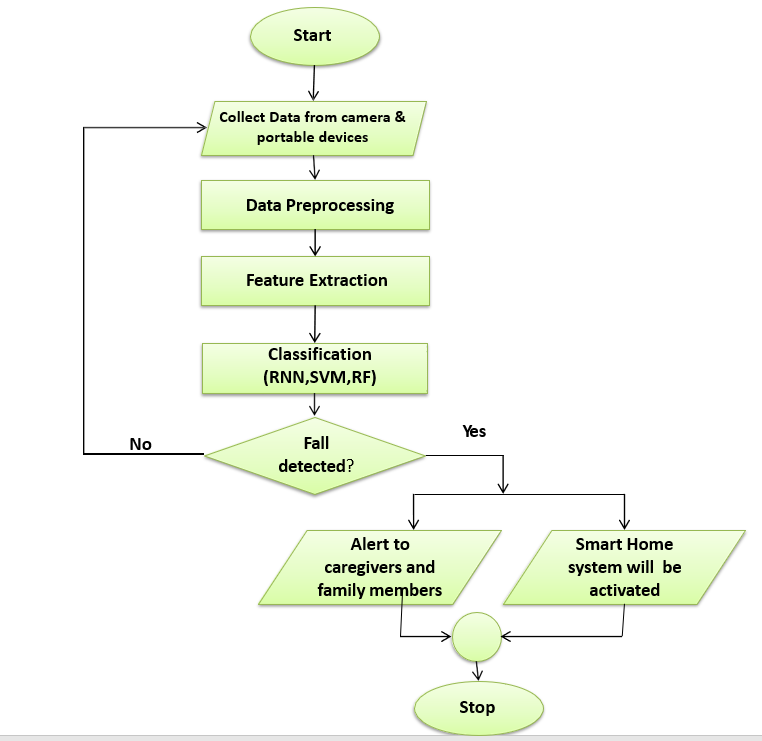
\includegraphics[width=4.2in]{Chap3/flowchart of fall detection.PNG}
%   \caption{Flow chart of Fall detection }
%   \label{fig:fall detection}
%     \end{figure}

% \subsection{Detecion of Facial Expression}
% Figure \ref{fig:model} shows the flowchart of how image frames will be extracted from video sequences and facial expression will be detected. With an Attention system, the picture is first partitioned into a few sections, and we figure with a Convolutional Neural Network (CNN) portrayals of each part. At the point the consideration system is zeroing in on the applicable piece of the picture, so the decoder just uses explicit pieces of the picture. We use this mechanism in our project to identify the facial expression correctly wheather it is sad or happy or confused to understand the state of the patients via connecting cameras.

% MTCNN is a neural network which detects faces and facial landmarks on images. We use images and videoes in our project where we use this algorithm. MTCNN detects one or more faces from the image and extract its features to classify the face perfectly. The optimization of the image classification will be done by SVM but it doesn’t have its own classifier mechanism. By this reason we also combined it with the RF classifiers which is a learning algorithm and makes decision trees that tells us the final output. 
% \begin{figure}[H]
%   \centering
%   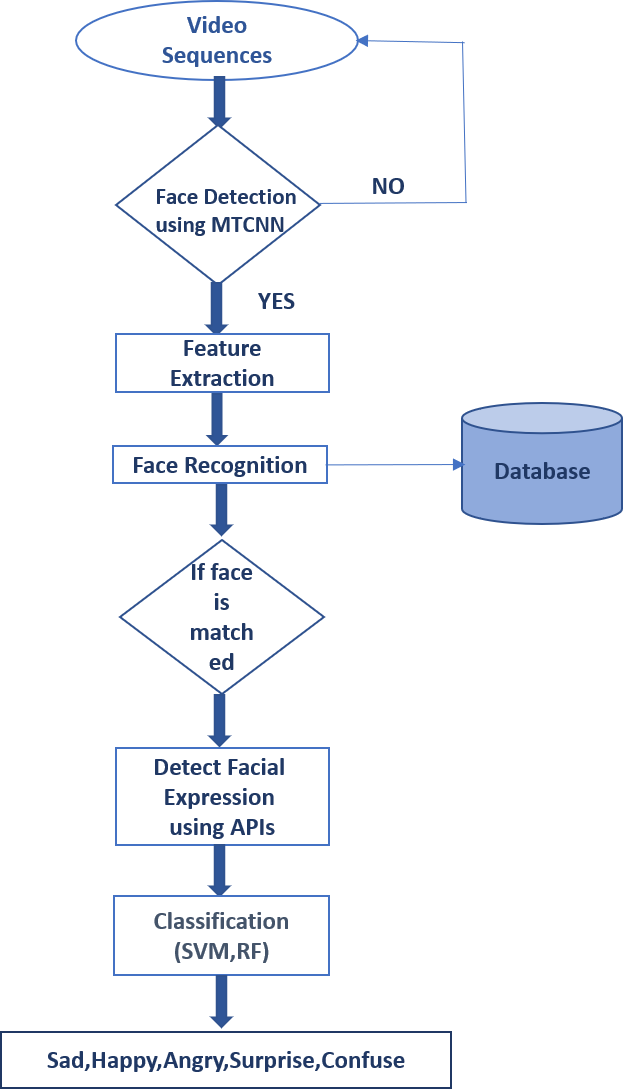
\includegraphics[width=4.2in]{Chap3/facial expression.png}
%   \caption{Flow chart of Facial Expression Extraction}
%   \label{fig:model}
%     \end{figure}
% Here the collected data set like video sequences will be given as input. The attention RNN mechanism will first detect the face and extract the features like context vector and attention weight and recognise the face wheather its happy or sad or angry or surprise or confused using APIs.


%\section{Dataset}
% \section{Dataset Description}
% Two datasets named 
% UR dataset and Open 
% labeled dataset have been
% used in our system 
% (see Table \ref{resulttab:1}).
% UR fall detection dataset are developed by kepski 
% \emph{et al.}
% \cite{kwolek_human_2014}
% used seventy sequences
% where thirty are falls 
% and fourty are activities 
% of daily living (ADL).
% Two camera are used.
% One is front facing 
% and other is from 
% ceiling which provides 
% the top views of the scene. Kinect cameras and corresponding accelerometric data are used to record fall and one device(camera 0) are used to record ADL. IMU and PS Move devices are used to collect sensor data. Two types of falls, one from standing and other while sitting on a chair are described here. Besides picking object from ground, lying on the sofa and floor, normal walking, sitting down are the ADL. Data needed to extract features of UR are\\
% \begin{itemize}
%     \item \textbf{Height/Width}- Bounding box height to width ratio
%     \item \textbf{l/w} - Major to minor axis ratio
%     \item \textbf{H/Hmax} - A proportion expressing the height of the person's surrounding box in the current frame to the physical height of the person, projected onto the depth map  and
%     \item \textbf{Area} - A ratio expressing the person’s area in the image to the area at assumed distance to the camera.
% \end{itemize} 

% Wertner \emph{et al.} \cite{wertner_open_2015} has created a labelled dataset which can be used for mobile phone with the data of accelerometer and gyroscope sensor. An orientation software based sensor is used to derive data from the accelerometer and geomagnetic field sensor which is attached to the mobile phone and the data is recorded by the mobile phone. Data needed to extract features of Open labelled are:

% \begin{itemize}
%     \item \textbf{Acceleration of devices:} Acceleration is stored as 3D vector indicating acceleration along each device axis, not including gravity. It can be calculated as
%     \begin{equation}
%         a_{xyz}=\sqrt{x^2+y^2+z^2}
%     \end{equation}
    
%      \item \textbf{Orientation of devices:} Orientation is stored as 3D vector of angles azimuth, pitch and roll.
% \end{itemize}


% \begin{figure}[!ht]
%     \centering
%     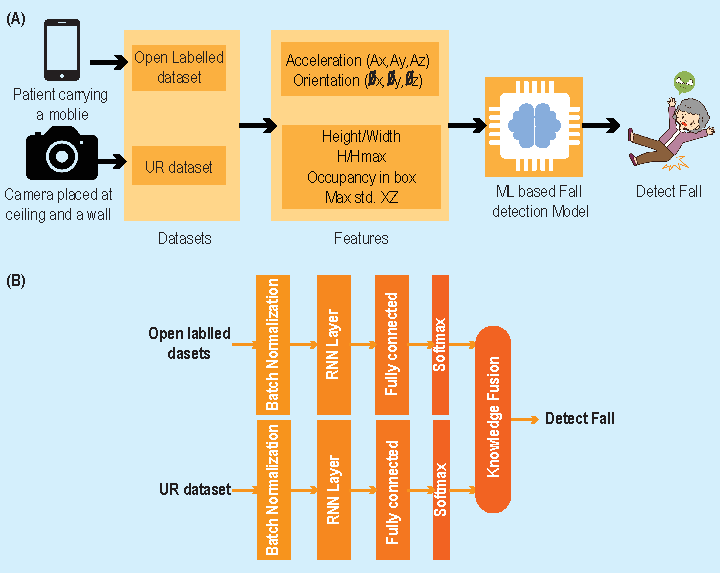
\includegraphics[scale=1.0]{Chap5/Fig03 B245.pdf}
%     \caption{Proposed Fall Detection Architecture and datasets used to train the model. (A) shows features used in the proposed RNN model and (B) illustrate the RNN architecture}
%     \label{fig:Fall_model}
% \end{figure}


% \begin{table}[!ht]
%     \centering
%     \scriptsize
%     \begin{tabular}{lp{1in}p{1.5in}cc}\toprule
%         Dataset & Sensor used &No of record & Training & Testing\\ \midrule
%          Open Labelled
% & Smart phone  &159300 records of acceleration
% and 159300 records of orientation&223020 &95580\\ \midrule
%         UR & Camera &70 (30 falls and 40 activities of daily living) sequences& 49&21\\ \bottomrule
%     \end{tabular}
%     \caption{Information about the dataset used in this study.}
%     \label{resulttab:1}
% \end{table}

\section{ML Algorithm}
The Machine Learning algorithm converts the data streams into actionable insight or detect anomaly from the data which are in the cloud. The information which are extracted from the data streams can be sent to patient's personal doctor, family members or the caregivers. This section describes ML algorithms briefly that has been used in the system model.We have used 3 Classifiers in our works. They are Random Forest (RF), Support Vector Machine (SVM), and Recurrent Neural Network (RNN). They are briefly described below: 

\subsection{RNN}
A Recurrent Neural Network(RNN) is an intrinsic
memory speculation of a feedforward neural network. RNN is very much useful in modeling the sequence data. Machine Translation, Time series prediction, Rhythm learning are the basic field for RNN.  It is sporadic in design since it has a comparable potential for each information contribution, although the latest information yield depends on the previous estimate. It is repeated and sent back into the
repeating networks in the aftermath of providing the yield. For settling on a option, it takes the current information and the yield that RNN has gained from the previous information. Figure \ref{fig:RNN} shows the basic diagram of Recurrent Neural Network.

\begin{figure}[ht]
    \centering
    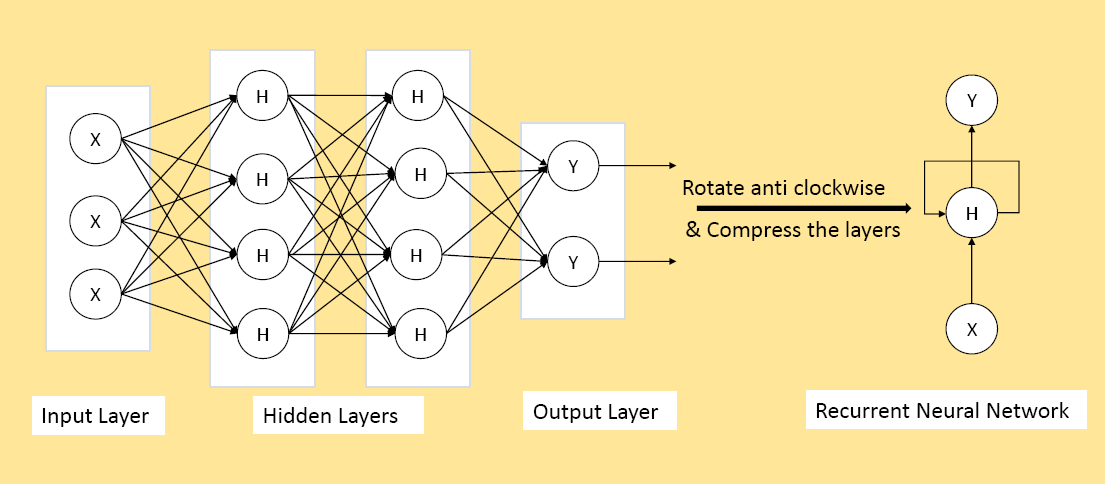
\includegraphics[scale=0.5]{Chap3/RNN.PNG}
    \caption{Recurrent Neural Network Layers}
    \label{fig:RNN}
\end{figure}

\vspace{.5cm}
%\subsubsection{Why Using LSTM instead of RNN}
All RNNs have criticism circles in the repetitive layer. This allows them to keep up data in 'memory' over the long run. Yet, it tends to be hard to prepare standard RNNs to take care of issues that require learning long haul worldly conditions. This is on the grounds that the inclination of the misfortune work rots dramatically with time (called the evaporating slope issue). LSTM networks are a sort of RNN that utilizes extraordinary units, notwithstanding standard units. LSTM units incorporate a 'memory cell' that can keep up data in memory for significant stretches of time. A bunch of doors is utilized to control when data enters the memory when it's yield, and when's it slipped its' mind. This engineering allows them to learn longer-term conditions.

\subsection{LSTM}
Long Short-Term Memory is an uncommon sort of RNN, fit for learning long term conditions. LSTM network is a changed adaptation of recurrent neural network, which made it simpler to regain past information in the memory. The problem of vanishing gradient issue introduced in RNN is solved here. In view of unwanted period delays, LSTM is ideal to define, quantify and forecast time arrangements. Back-propagation is used to prepare the models used in LSTM. Figure \ref{fig:lstm} shows the basic diagram of LSTM. There are three gates in an LSTN network. They are Input gate, Forget gate and Output gate. They are described below: 
 \begin{enumerate}
     \item \textbf{Input Gate: } This gate finds which data value from information need to be used to adjust memory of the system. Sigmoid capacity decides which data needs  to let through 0 or 1. Also, The tanh function is used here, which gives weight to the characteristics that are transferred choosing their degree of meaning from-1 to 1.
     
     \item \textbf{Forget Gate: } This gate finds the subtleties to be extracted from the block. The sigmoid function choose it. This gate takes a gander at the previous state which is described by (Ht-1) and the substance input denoted by (Xt) and yields a number between 0( Which means omit this ) and 1( which means keep this ) for each number in the cell state denoted by Ct-1.
     
     \item\textbf{Output Gate: } Output is choosed by the utilization of information and the memory of the block. Sigmoid capacity decides here which data streams need to let through 0,1. Moreover, tanh function offers weightage to the qualities which are passed through it, decides their degree of significance ranging from-1 to 1 and which is replicated with an output of Sigmoid function.
 \end{enumerate}
% Figure \ref{fig:lstm2} shows the lstm layers.
  \begin{figure}[ht]
    \centering
    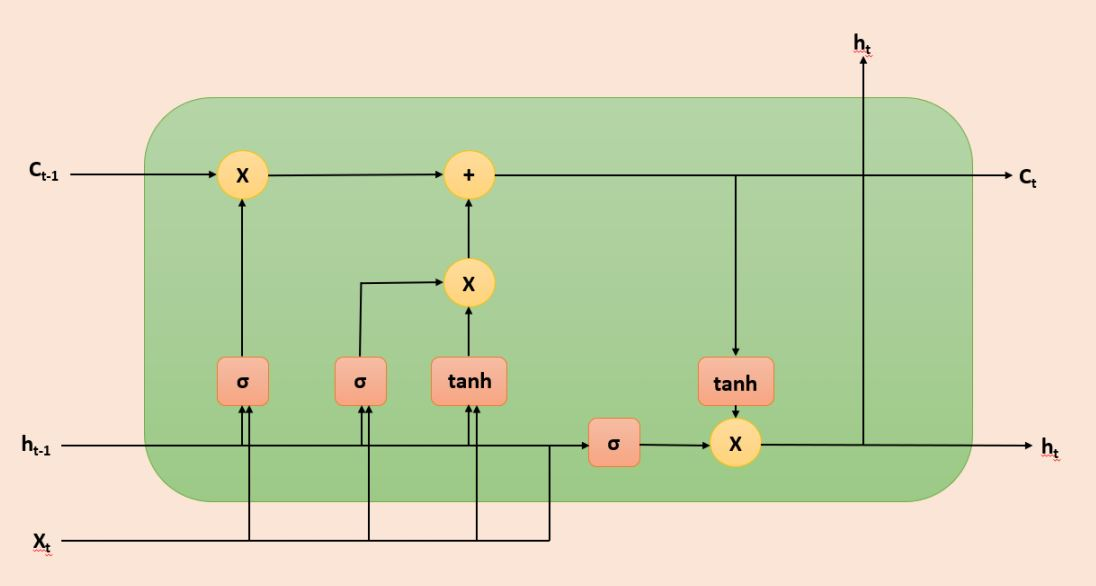
\includegraphics[scale=0.4]{Chap3/LSTN.JPG}
    \caption{LSTM gates}
    \label{fig:lstm}
\end{figure}
% Figure \ref{fig:lstmfall2} shows the architecture of lstm layers to detect a fall activity.
% \begin{figure}[!ht]
%     \centering
%     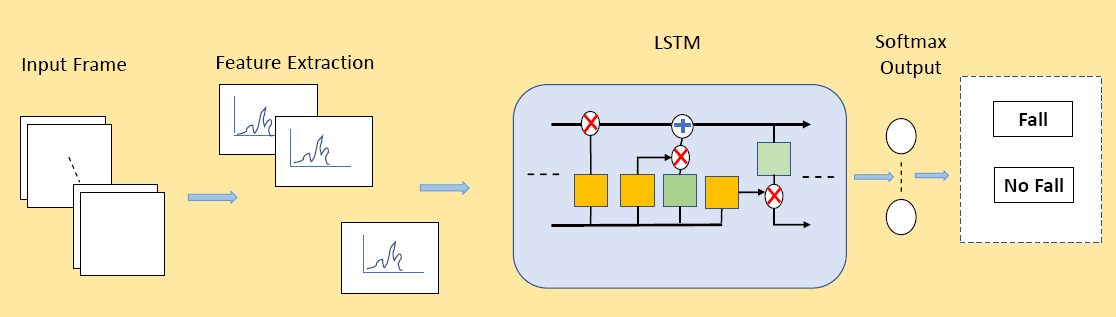
\includegraphics[scale=0.4]{Chap3/lstmFall.PNG}
%     \caption{LSTM layer for fall detection}
%     \label{fig:lstmfall2}
% \end{figure}

% \begin{figure}[ht]
%     \centering
%     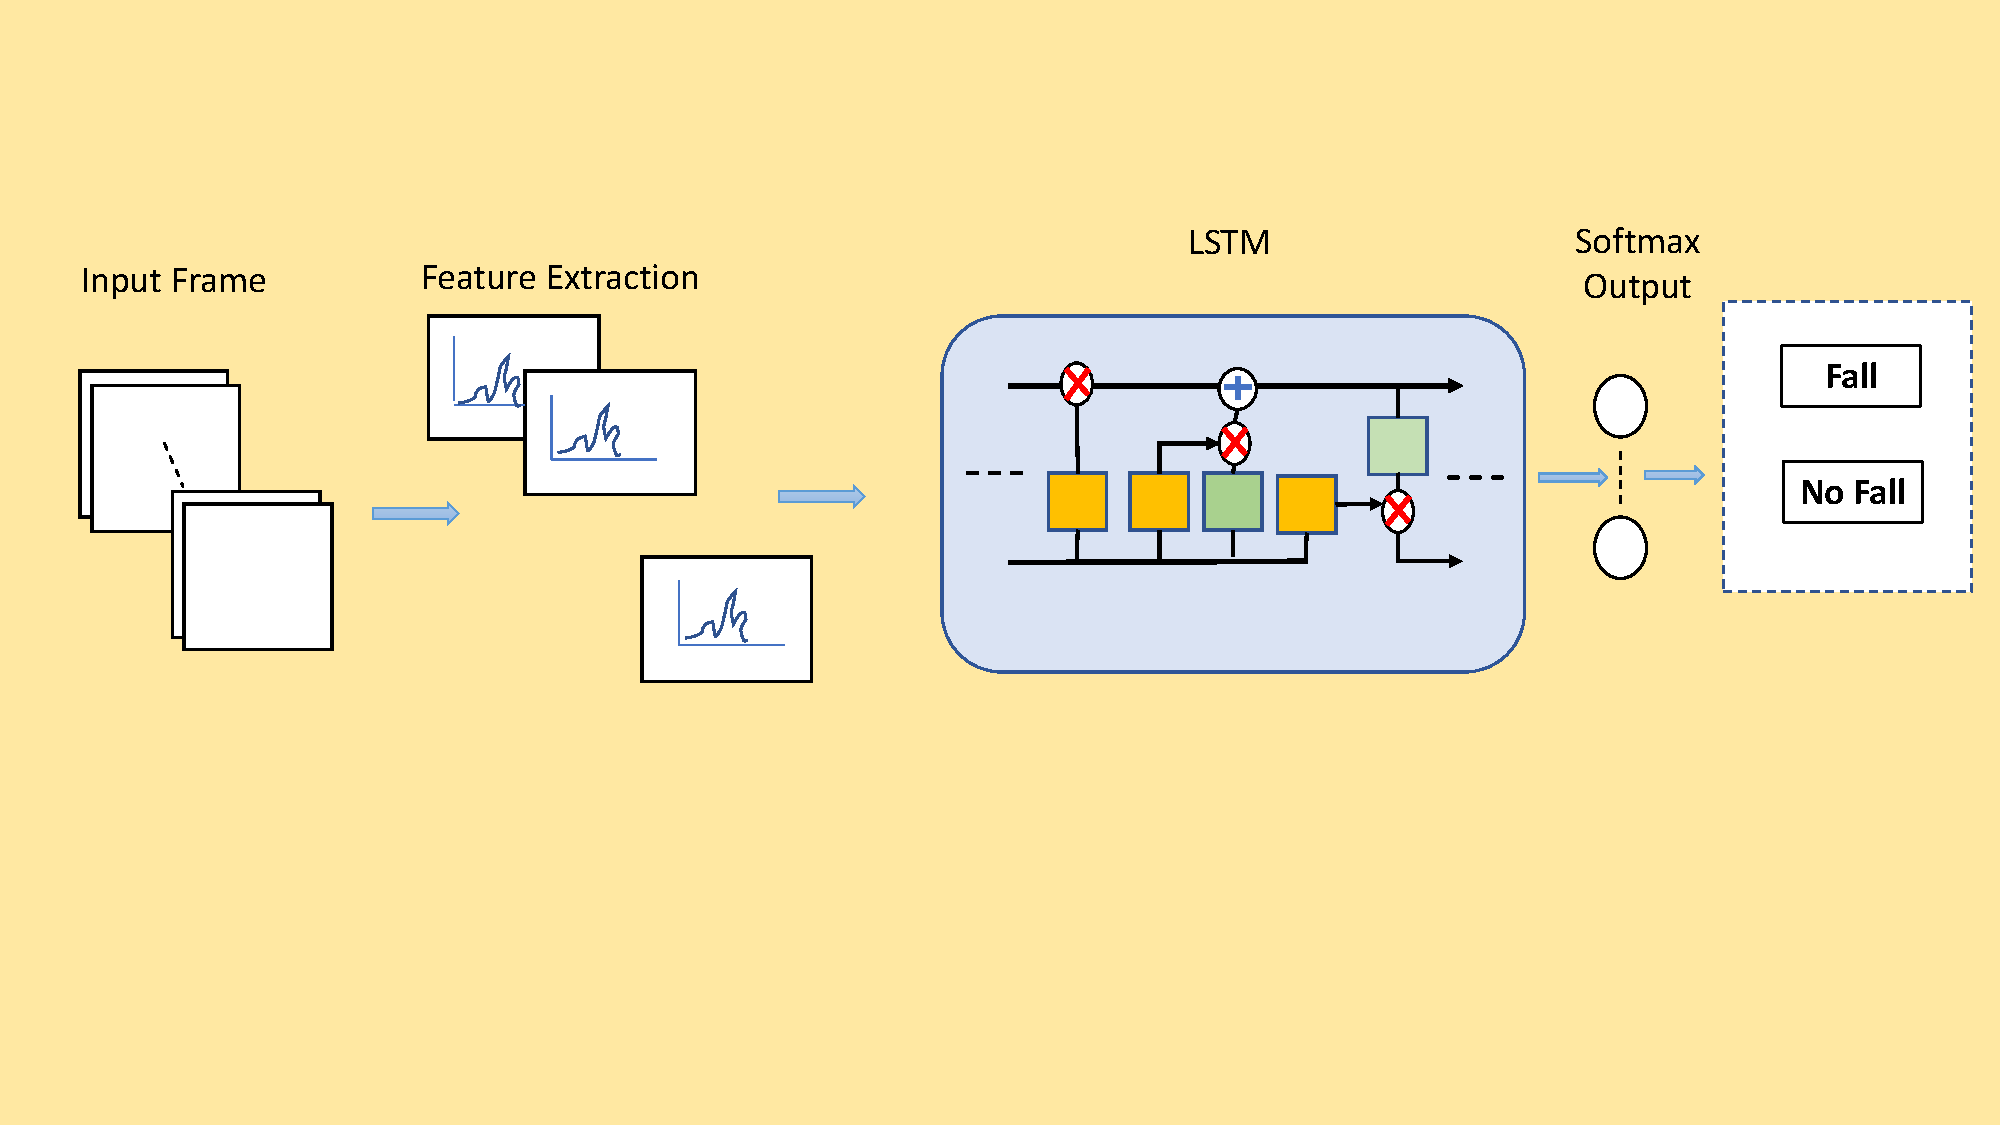
\includegraphics[scale=0.5]{Chap3/LSTM2.pdf}
%     \caption{LSTM layers}
%     \label{fig:lstm2}
% \end{figure}

\subsection{Random Forest (RF):}Random forest is a classification algorithm that is a set of decision trees where a group
of decision trees build a tree forest to maximize the total outcome by integrating learning models. The input of Random Forest is evaluated by the decision tree forest and the response tree class is considered as the output class of Random Forest. Random Forest is user friendly machine learning algorithm as it is easy to use. The forest this algorithm builds is a combination of decisions trees which is trained  by the
"Bagging" method where bagging indicates the combination of learning models which will increase the overall result.  It produce a great result most of the time comparing to other machine learning algorithm. Figure \ref{fig:RF} Shows the basic Random forest diagram of how it works. Another wonderful benefit of the random forest algorithm is that the relative
significance of each function of the forecast is very simple to calculate. If we insert a training set with attributes and labels into a random forest,
any set of rules that is used to make the decisions will be formulated. 
\begin{figure}[ht]
    \centering
    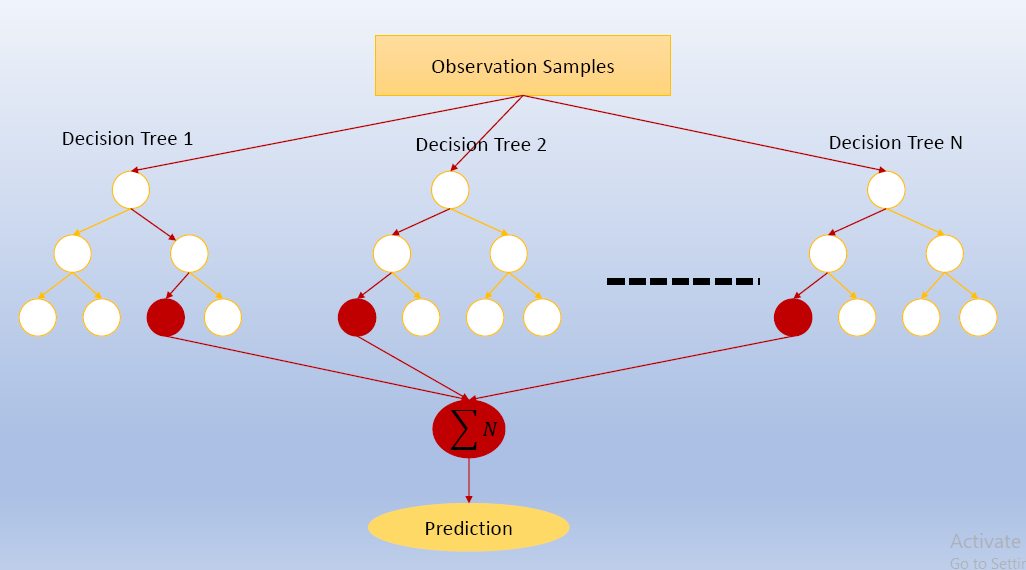
\includegraphics[scale=0.5]{Chap3/RF.PNG}
    \caption{Random Forest}
    \label{fig:RF}
\end{figure}

\subsection{Support Vector Machine (SVM):} The support vector machine (SVM) is a supervised ML
model that utilizes classification algorithms to solve two-group classification problems.. They will categorize fresh text that has an SVM model collection of named training details in every unit. The aim of the support vector machine algorithm seems to be discover a hyper-plane that separately categorizes the points in an N-dimensional range (N-the number of features). Hyper-planes are boundaries of decisions to identify the data points. Various groups can be related to data points falling on each side of the hyper-plane. The hyper-plane's dimension based on the quantity of Input characteristics. When the input is 2, it’s a line in hyper-plane and when it comes in 3 it becomes a two-dimensional in the hyper-plane. When the number of functions reaches 3, it becomes impossible to visualize.  The nearest hyper-plane is the support vectors which are also one kind of data points as well as impact the hyper-plane's direction and context. Use these support vectors to expand the range of the classifier. Selecting the support vectors may alter its direction of hyper - plane.

\vspace{0.5cm}
The support vectors are the data points nearest to single hyper-plane; these shall be beyond the boundaries of the section. The accompanying figure reflects these definitions, with + demonstrating information purposes of type 1, and – showing information purposes of type – 1. Figure \ref{fig:SVM} shows the basic procedure of Support vector Machine.

\begin{figure}[!ht]
    \centering
    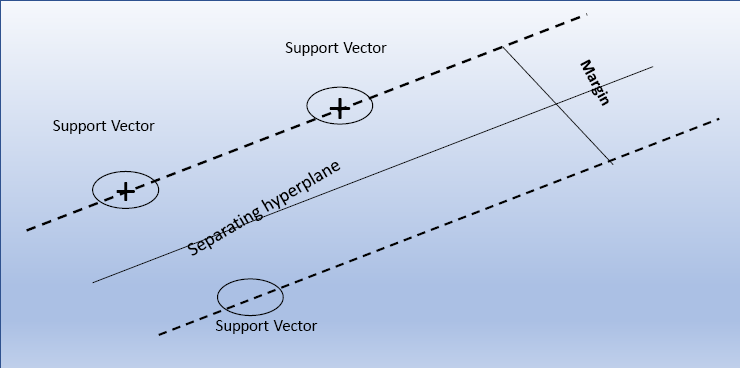
\includegraphics[scale=0.7]{Chap3/SVM.PNG}
    \caption{Support Vactor Machine}
    \label{fig:SVM}
\end{figure}

% We are trying to make a dataset as per required for our model. Collecting data using camera and video sensors to make a proper dataset for the management of NDDs. We are trying to attempt for finding some ND patients and collect some real-time data to make a real-time dataset for our project.

% \section{Research Timeline}
% \begin{figure}[H]
%   \centering
%   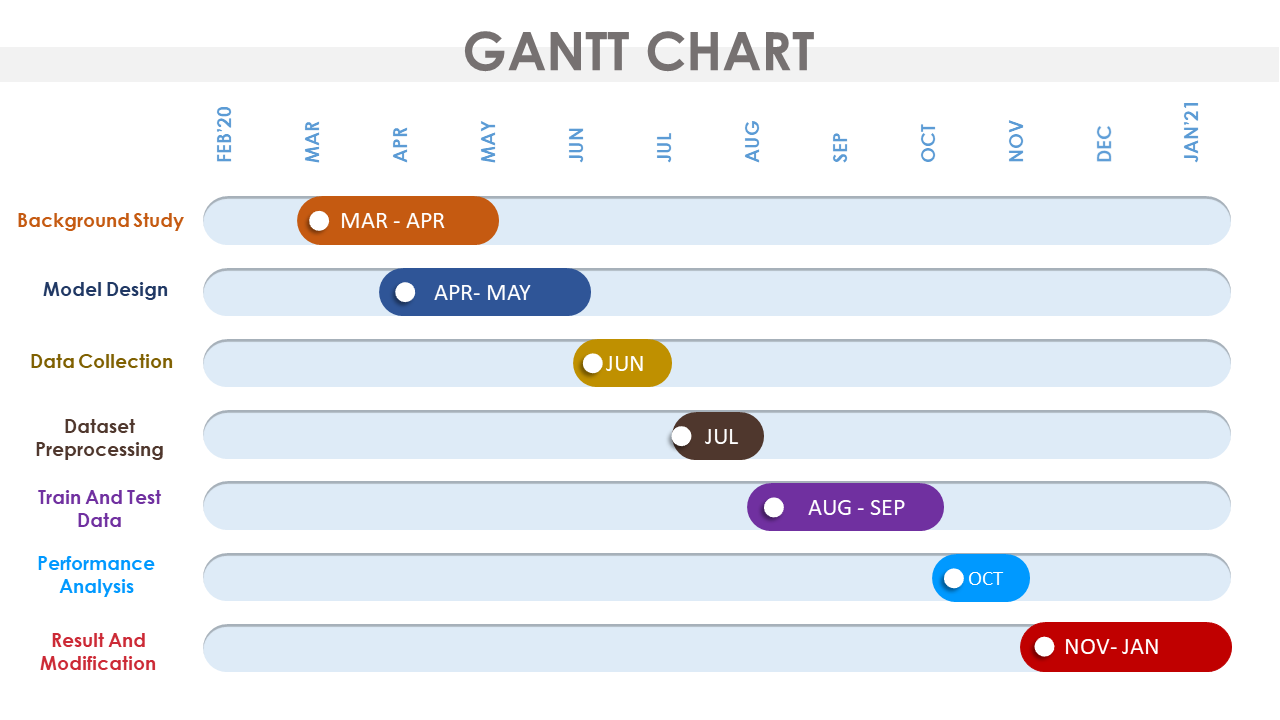
\includegraphics[width=6.2in]{Chap3/gantt_chart.png}
%   \caption{Research Timeline of Management of Nuerodegenarative Disease using Machine Learning and Internet of Things }
%   \label{fig:ganttchart}
%     \end{figure}
% Figure \ref{fig:ganttchart} illustrates our research timeline. Here we have listed our tasks to be performed on the vertical axis, and time interval is listed on the horizontal axis. The width of the horizontal bars indicates the duration of our activities.